\documentclass{article}
\usepackage[utf8]{inputenc}
\usepackage{mytex}
\usepackage{placeins}

\title{
    \normalsize \textsc{} \\[2.0cm]
    \HRule{1pt} \\[0.3cm]
    \LARGE \textbf{Principles of Database Systems (CS6083)}
    \HRule{1pt} \\[0.5cm]
    \Large Project 1 \\[0.5cm]
    \normalsize \today
}

\author{
    Mingyu Zhao, Hangbo Fan \\
    New York University \\
    Tandon School of Engineering \\
    \texttt{m.zhao@nyu.edu}, \texttt{hf9292@nyu.edu} \\
}

\begin{document}

\thispagestyle{empty}
\printtitle%
      \vfill
\printauthor%
\newpage

\section{Introduction}

\subsection{Assumption}
We have the following assumptions when designing our system:
\begin{enumerate}
    \item Each email address can only be used to register one account, and users will not be about to change their email since signed up. After created an account, users will login with their email address and password.
    \item The \textit{wmtype} shows the role of the member which is either administrator or user in the \textbf{Workspace}.
    \item Because a user cannot send two messages in the same channel of the sam workspace at a single second, we use (\textit{wid}, \textit{cname}, \textit{uemail}, \textit{mtime}) as the primary key of the \textbf{Message} relation.
    \item Instead of using trigger in our database, we will use multiple SQL statements if cascading operations are needed.
\end{enumerate}


\section{Entity-Relationship Model}
Our entity-relationship diagram is modeled as follows:

\begin{figure}[ht!]
    \centering
    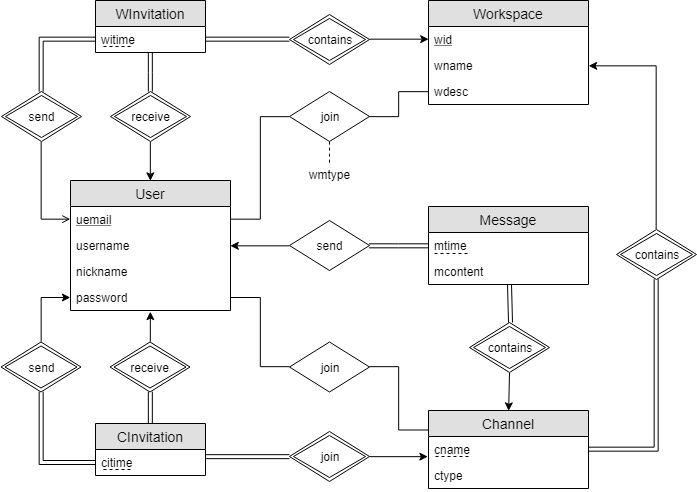
\includegraphics[width=0.8\textwidth]{img/erd.png}
    \caption{Entity-Relationship Diagram}
\end{figure}

Here, the \textbf{Message}, \textbf{Channel}, \textbf{CInvitation} and \textbf{WInvitation} become weak entities. And the \textbf{join} relationship between \textbf{User} and \textbf{Workspace} has an attribute \textit{wmtype}, indicating the user in a particular workspace is an administrator or a coworker.

\newpage


\section{Relational Schema Design}

Translating from the entity-relationship model, we have the following relational schema (the underlined attributes are chosen as the primary keys):
\begin{itemize}
    \item \textbf{User} (\underline{uemail}, username, nickname, password)
    \item \textbf{Workspace} (\underline{wid}, wname, wdesc)
    \item \textbf{Channel} (\underline{wid}, \underline{cname}, ctype, ctime)
    \item \textbf{Message} (\underline{wid}, \underline{cname}, \underline{uemail}, \underline{mtime}, mcontent)
    \item \textbf{WInvitation} (\underline{semail}, \underline{remail}, \underline{wid}, \underline{witime})
    \item \textbf{CInvitation} (\underline{semail}, \underline{remail}, \underline{wid}, \underline{cname}, \underline{citime})
    \item \textbf{WMember} (\underline{uemail}, \underline{wid}, wmtype)
    \item \textbf{CMember} (\underline{uemail}, \underline{wid}, \underline{cname})
\end{itemize}

\smallskip

And we also have foreign key constraints among these relations:
\begin{itemize}
    \item \textit{wid} is a foreign key from \textbf{Channel}, referencing \textbf{Workspace}
    \item (\textit{wid}, \textit{cname}) is a foreign key from \textbf{Message}, referencing \textbf{Channel}
    \item \textit{uemail} is a foreign key from \textbf{Message}, referencing \textbf{User}
    \item \textit{semail} is a foreign key from \textbf{WInvitation}, referencing \textbf{User}
    \item \textit{remail} is a foreign key from \textbf{WInvitation}, referencing \textbf{User}
    \item \textit{wid} is a foreign key from \textbf{WInvitation}, referencing \textbf{Workspace}
    \item \textit{semail} is a foreign key from \textbf{CInvitation}, referencing \textbf{User}
    \item \textit{remail} is a foreign key from \textbf{CInvitation}, referencing \textbf{User}
    \item (\textit{wid}, \textit{cname}) is a foreign key from \textbf{CInvitation}, referencing \textbf{Workspace}
    \item \textit{uemail} is a foreign key from \textbf{WMember}, referencing \textbf{User}
    \item \textit{wid} is a foreign key from \textbf{WMember}, referencing \textbf{Workspace}
    \item \textit{uemail} is a foreign key from \textbf{CMember}, referencing \textbf{User}
    \item (\textit{wid}, \textit{cname}) is a foreign key from \textbf{CMember}, referencing \textbf{Channel}
\end{itemize}

\smallskip

The visualized relational schema is also shown below:
\begin{figure}[ht!]
    \centering
    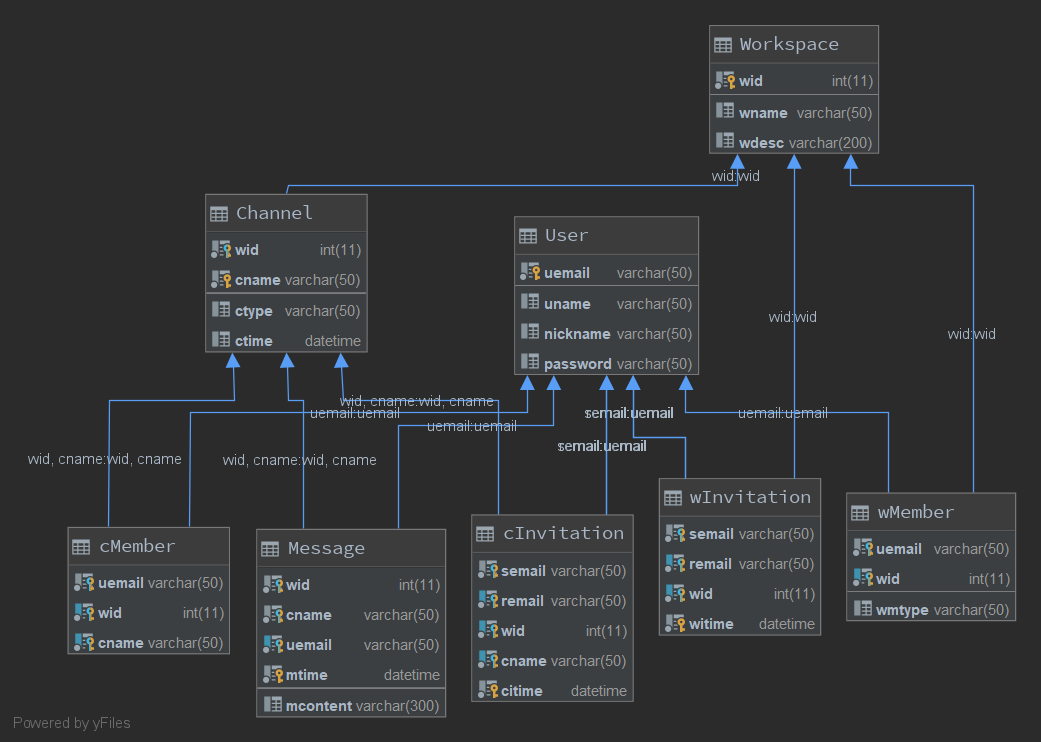
\includegraphics[width=0.8\textwidth]{img/relation-schema.png}
    \caption{Visualized Relational Schema}
\end{figure}

\newpage

\import{parts/}{implementation.tex}

\end{document}
